\documentclass[journal,12pt,twocolumn]{IEEEtran}
\usepackage{./report_macros}

\begin{document}
\vspace{3cm}
\title{Quick UnbIased Compression for Federated Learning (QUIC-FL): A Report}
\author{Gautam Singh\\CS21BTECH11018}
\maketitle
\tableofcontents
\bigskip

\begin{abstract}
    This document is a report of the paper \cite{basat2023quicfl}. It 
    summarizes the main contributions of the authors and analyzes the results
    obtained. This report also lists out possible future research in the area
    of Federated Learning (FL).
\end{abstract}

\section{Problem Statement}
\label{sec:ps}
The authors of \cite{basat2023quicfl} consider the \textbf{Distributed Mean 
Estimation} problem, illustrated in \autoref{fig:dme}. Specifically, each 
client \(C_i\) sends data \(\vect{x}_i\), quantized as \(\vect{Y}_i\in
\cbrak{0,1}^b\), for \(1 \le i \le n\). Here, \(b\) represents the number
of bits used for quantization per client.

\begin{figure}[!ht]
    \begin{tikzpicture}[node distance = 5ex]
    \node[state] (C_1) {$C_1$}; 
    \node[state] (C_2) [right=of C_1] {$C_2$}; 
    \node (L) [right=of C_2] {$\ldots$};
    \node[state] (C_n) [right=of L] {$C_n$}; 
    \node[state,rectangle] (S) [above=of $(C_2.north)!0.5!(L.north)$] {$S$};
    \node (X_1) [below=of C_1] {$\vect{X_1} \in \bR^d$};
    \node (X_2) [below=of C_2] {$\vect{X_2}$};
    \node (X_n) [below=of C_n] {$\vect{X_n}$};
    \node (L1) [below=of L] {$\ldots$};
    \node (muhat) [above=of S] {$\hat{\vect{\mu}} \triangleq \frac{1}{n}\sum_{i=1}^n\hat{\vect{X_i}}$}; 
    \path[->]
    (C_1) edge  node [left=1ex] {$\vect{Y_1} \in \cbrak{0,1}^b$} (S)
    (C_2) edge  node [right=1ex] {$\vect{Y_2}$} (S)
    (C_n) edge  node [right=1ex] {$\vect{Y_n}$} (S)
    (S) edge node {} (muhat)
    (X_1) edge node {} (C_1)
    (X_2) edge node {} (C_2)
    (X_n) edge node {} (C_n);
\end{tikzpicture}
    \caption{An Illustration of the DME Problem.}
    \label{fig:dme}
\end{figure}

The server computes the estimates \(\hat{\vect{X}}_i\) using the obtained 
\(\vect{Y}_i\) as
\begin{equation}
    \hat{\vect{\mu}} \triangleq \frac{1}{n}\sum_{i=1}^n\hat{\vect{X}}_i.
    \label{eq:muhat-def}
\end{equation}

The aim of the DME problem is to estimate the true mean \(\vect{\mu} \triangleq
\frac{1}{n}\sum_{i=1}^n\vect{X}_i\) using \(\hat{\vect{\mu}}\) as defined in
\eqref{eq:muhat-def} with \emph{minimal error} (see \autoref{ssec:nmse}).

\section{Goals of the Paper}
\label{sec:goals}
The goals of \cite{basat2023quicfl} are to develop a quantization scheme that,
compared to other state-of-the-art methods (see \autoref{ssec:res-comp} for a 
list of such methods).

\begin{enumerate}
    \item Less computational complexity compared to other methods, at 
    \emph{both} client and server.
    \item Same (asymptotic) NMSE of \(\cO\brak{\frac{1}{n}}\).
    \item Same convergence rate.
    \item Better compression ratio.
\end{enumerate}

\section{Preliminaries}
\label{sec:prelims}
\subsection{vNMSE and NMSE}
\label{ssec:nmse}
The main performance metric used to assess a quantization scheme is the
\emph{squared error} of the estimated mean from the actual mean. To perform
such an assessment, the authors define two quantities that will be useful.
\begin{definition}[vNMSE]
    \label{def:vnmse}
    The \emph{vector Normalized Mean Square Error} of a vector \(\vect{x}\)
    is defined as
    \begin{equation}
        vNMSE \triangleq \frac{\mean{\norm{\hat{\vec{x}}-\vec{x}}^2_2}}{\norm{\vect{x}}^2_2}.
        \label{eq:vnmse-def}
    \end{equation}
\end{definition}
\begin{definition}[NMSE]
    \label{def:nmse}
    For the DME problem, the \emph{Normalized Mean Square Error} is defined
    as
    \begin{align}
        NMSE &\triangleq \frac{\mean{\norm{\hat{\vect{\mu}}-\vect{\mu}}^2_2}}{\frac{1}{n}\sum_{i=1}^n\norm{\vect{x}_i}^2_2} \\
        &= \frac{\mean{\norm{\hat{\vect{\mu}}-\frac{1}{n}\sum_{i=1}^n\vect{x}_i}^2_2}}{\frac{1}{n}\sum_{i=1}^n\norm{\vect{x}_i}^2_2}.
        \label{eq:nmse-def}
    \end{align}
\end{definition}
From \autoref{def:vnmse} and \autoref{def:nmse}, we can perform simple 
algebraic manipulations to obtain the following result.
\begin{lemma}
    \label{lem:vnmse-nmse-rel}
    For \(n\) clients with unbiased and independent estimates, we have
    \cite{EDEN}
    \begin{equation}
        NMSE = \frac{\sum_{i=1}^nvNMSE\brak{i}\norm{\vect{x}_i}_2^2}{n\sum_{i=1}^n\norm{\vect{x}_i}_2^2}
        \label{eq:vnmse-nmse-rel}
    \end{equation}
\end{lemma}
\begin{proof}
    \label{proof:vnmse-nmse-rel}
    From \eqref{eq:nmse-def}, we obtain
    \begin{align}
        NMSE &= \frac{\mean{\norm{\sum_{i=1}^n\brak{\hat{\vect{x}}_i - \vect{x}_i}}_2^2}}{n\sum_{i=1}^n\norm{\vect{x}_i}_2^2} \\
        &= \frac{\sum_{i=1}^n\mean{\norm{\hat{\vect{x}}_i - \vect{x}_i}_2^2}}{n\sum_{i=1}^n\norm{\vect{x}_i}_2^2} \label{eq:lem-step1} \\
        &= \frac{\sum_{i=1}^nvNMSE\brak{i}\norm{\vect{x}_i}_2^2}{n\sum_{i=1}^n\norm{\vect{x}_i}_2^2}. \label{eq:lem-step2}
    \end{align}
    where \eqref{eq:lem-step1} is due to the fact that the estimates are
    unbiased and independednt, thus eliminating cross terms, and
    \eqref{eq:lem-step2} is by \eqref{eq:vnmse-def}.
\end{proof}
We also obtain this simple corollary as a result of \eqref{eq:lem-step2}.
\begin{corollary}
    \label{cor:vnmse-equal}
    In \autoref{lem:vnmse-nmse-rel}, if all clients have the same \(vNMSE\)
    which is independent of the L2-norm of its vector, then
    \begin{equation}
        NMSE = \frac{vNMSE}{n}.
        \label{eq:nmse-vnmse-eq}
    \end{equation}
\end{corollary}
\subsection{Randomized Hadamard Transform (RHT)}
\label{ssec:rht}
QUIC-FL uses the RHT to gain speed asymptotically. In this subsection, we
present a few definitions and important properties of the RHT.

\begin{definition}[Walsh-Hadamard Matrix]
    \label{def:wh-matrix}
    The Walsh-Hadamard matrix \(\vect{H}_{2^k}\) with \(\vect{H}_1 = 
    \myvec{1}\) is recursively defined as
    \begin{equation}
        \vect{H}_{2^k} = \myvec{\vect{H}_{2^{k-1}} & \vect{H}_{2^{k-1}} \\ \vect{H}_{2^{k-1}} & -\vect{H}_{2^{k-1}}}.
        \label{eq:Hl-def}
    \end{equation}
\end{definition}
\begin{definition}[Randomized Hadamard Transform]
    \label{def:rht}
    Let \(\vect{H}\in\cbrak{-1,+1}^{d\times d}\) be a Walsh-Hadamard 
    Matrix and \(\vect{D}\) be a diagonal matrix with uniform iid 
    Rademacher entries \emph{i.e.}, entries that are \(\pm 1\) with 
    equal probability. Then, the \emph{randomized Hadamard transform} 
    (RHT) of \(\vect{x}\in\bR^d\) is given by
    \begin{equation}
        \cR_{\vect{H}}\brak{\vect{x}} \triangleq \brak{\frac{1}{\sqrt{d}}\vect{HD}}\vect{x}.
        \label{eq:rht-def}
    \end{equation}
\end{definition}
We can also define the inverse of the transform as follows.
\begin{definition}[Inverse RHT]
    The \emph{inverse randomized Hadamard transform} of \(\vect{x}\) is
    given by
    \begin{equation}
        \cR_{\vect{H}}^{-1}\brak{\vect{x}} \triangleq \brak{\frac{1}{\sqrt{d}}\vect{DH}}\vect{x}.
        \label{eq:inv-rht-def}
    \end{equation}
\end{definition}
A key property of the RHT is obtained in the limit that \(d\to\infty\),
which we state without proof.
\begin{theorem}
    \label{thm:rht-norm-conv}
    Define \(F_{i,d}\brak{x}\) to be the CDF of the random variable
    \(\frac{1}{\sigma}\cR_{\vect{H}}\brak{\vect{x}}_i\), where
    \(\mean{x_i^2} = \sigma^2\), and \(\Phi\brak{x}\) the CDF of the
    standard normal distribution. Then, as \(d\to\infty\), \(\forall\ 1 \le
    j \le d\), 
    \begin{equation}
        F_{i,d}\brak{x_j} \xrightarrow{\mathrm{d}} \Phi\brak{x_j}.
        \label{eq:rht-norm-conv}
    \end{equation}
\end{theorem}
\autoref{thm:rht-norm-conv} establishes a weak convergence between the RHT
and the standard normal distribution, which is important for QUIC-FL, as we
shall see.
\section{Bounded Support Quantization (BSQ)}
\label{sec:bsq}
In this section, we describe the Bounded Support Quantization (BSQ) algorithm,
which is used in QUIC-FL. We then proceed to analyze its NMSE, and comment on
its utility. The BSQ encoding algorithm is described in \autoref{alg:bsq-enc}
and the BSQ decoding algorithm is described in \autoref{alg:bsq-dec}.
\begin{algorithm}[H]
    \caption{BSQ Encoder}
    \label{alg:bsq-enc}
    \begin{algorithmic}[1]
        \Require{BSQ parameter \(p\in\lbrak{\rsbrak{0,1}}\), stochastic
        quantization algorithm \(Q\).}
        \Procedure{BSQ-Encoder}{$\vect{x}$}
        \State $t_p \gets$ threshold such that at most \(dp\) points in
        \(\vect{x}\) lie outside \(\sbrak{-t_p, t_p}\).
        \State $\vect{U} \gets \cbrak{x_{i}\ |\ \abs{x_{i}} > t_p}$
        \State $\vect{I} \gets \cbrak{i\ |\ \abs{x_{i}} > t_p}$
        \State $\vect{V} \gets \cbrak{x_{i}\ |\ \abs{x_{i}} \le t_p}$
        \State $\vect{X} \gets Q\brak{\vect{V}}$.
        \State Output $\brak{\vect{U}, \vect{I}, \vect{X}}$.
        \EndProcedure
    \end{algorithmic}
\end{algorithm}

\begin{algorithm}[H]
    \caption{BSQ Decoder}
    \label{alg:bsq-dec}
    \begin{algorithmic}[1]
        \Require{BSQ parameter \(p\in\lbrak{\rsbrak{0,1}}\).}
        \Procedure{BSQ-Decoder}{$\vect{U},\vect{I},\vect{X}$}
        \State $\hat{\vect{X}} \gets$ reconstructed points from $\vect{X}$.
        \State $\hat{\vect{x}} \gets
        \textsc{Merge}\brak{\vect{U},\vect{I},\hat{\vect{X}}}$. 
        \State Output $\hat{\vect{x}}$.
        \EndProcedure
    \end{algorithmic}
\end{algorithm}

The BSQ parameter \(p\) is chosen by the designer. The essence of BSQ lies in
the fact that errors for larger components may incur a larger NMSE. Thus, by
quantizing in a \emph{bounded support} \(\sbrak{-t_p,t_p}\), we can limit the
NMSE. The main result of BSQ stated without proof is given below.

\begin{theorem}
    \label{thm:bsq-nmse}
    BSQ, without further assumptions, admits a worst-case NMSE of
    \(\frac{1}{np\brak{2^b-1}^2}\) with \(\cO\brak{d}\) and \(\cO\brak{nd}\)
    complexity for encoding and decoding respectively.
\end{theorem}

One can clearly see that selecting arbitrarily small \(p\) can lead to a large
constant factor in the NMSE. QUIC-FL performs a random rotation of \(\vect{x}\)
before applying BSQ to bound this constant factor.

\section{Distribution-Aware Unbiased Quantization}
\label{sec:dauq}
The key idea of this quantization scheme lies in the fact that \(\forall\ 1 \le
i \le d\), where \(\vect{R}\) denotes a random rotation matrix
\cite{vargaftik2021drive},
\begin{equation}
    \frac{\sqrt{d}}{\norm{\vect{x}}_2}\brak{\vect{Rx}}_i \sim \cN\brak{0,1}.
    \label{eq:rot-norm-conv}
\end{equation}
Thus, we only need to optimize the reconstruction values for when the data is
sampled from the \emph{standard normal distribution}. This will yield a
\emph{near-optimal} quantization for the original vectors \(\vect{x}_i\). Notice
that this is possible since
\begin{enumerate}
    \item We know the distribution of the transformed vector by
    \eqref{eq:rot-norm-conv}, as well as the inverse transform.
    \item We know the bounded support range \(\sbrak{-t_p, t_p}\) in which
    stochastic quantization must be performed.
\end{enumerate}
Therefore, we can format this new quantization problem as an optimization
problem. The notation used for this section is shown in \autoref{tab:dauq-defs}.

\begin{table*}
    \centering
    \begin{tabular}{|c|c|}
        \hline
        \textbf{Notation} & \textbf{Definition} \\
        \hline
        \(p\) & BSQ parameter \\
        \hline
        \(t_p\) & BSQ threshold \\
        \hline
        \(b\) & Number of bits per quantized value \\
        \hline
        \(\cM\) & Message space \(\cbrak{0,1,\ldots,2^b-1}\) \\
        \hline
        \(R\brak{x}\) & Reconstruction point associated with \(x\) at the receiver \\
        \hline
        \(\cQ_{b,p}\) & Set of all reconstruction points \(\cbrak{R\brak{x}\ |\ x \in \cM}\) \\
        \hline
        \(\cI_m\) & \(\cbrak{0,1,\ldots,m-1}\) \\
        \hline
        \(\cA_{p,m}\brak{i}\) & \(\pr{Z \le \cA_{p,m}\brak{i}\ |\ Z \in \sbrak{-t_p,t_p},\ Z \sim \cN\brak{0,1}} = \frac{i}{m-1}\) \\
        \hline
        \(\cA_{p,m}\) & Right endpoints of quantiles \(\cbrak{\cA_{p,m}\brak{i}\ |\ i\in\cI_m}\) \\
        \hline
        \(S\brak{z,x}\) & \(\pr{z \text{ is quantized to } R\brak{x}}\) \\
        \hline
        \(S^\prime\brak{i,x}\) & \(S\brak{\cA_{p,m}\brak{i}, x}\) \\
        \hline
    \end{tabular}
    \caption{Notation for Distribution-Aware Unbiased Quantization.}
    \label{tab:dauq-defs}
\end{table*}

\subsection{The Optimization Problem}
\label{ssec:dauq-opt}
We want to minimize the MSE of this quantizer while keeping it unbiased. Thus,
the optimization problem for the distribution-aware unbiased quantizer is

\begin{align}
    \min_{S,R} \int_{-t_p}^{t_p} &\sum_{x\in\cM}S\brak{z,x}\brak{z-R\brak{x}}^2e^{-\frac{z^2}{2}}dz\ \label{eq:dauq-mse} \\
    \text{s.t (Probability)} &\sum_{x\in\cM}S\brak{z,x} = 1 \label{eq:dauq-prob} \\
    \text{(Unbiasedness)} &\sum_{x\in\cM}S\brak{z,x}R\brak{x} = z. \label{eq:dauq-unbias}
\end{align}

Notice that without the constraint in \eqref{eq:dauq-unbias}, this optimization
problem corresponds to that of the Lloyd-Max quantizer. 

\subsection{Discretization}
\label{ssec:dauq-disc}
The optimization problem in \eqref{eq:dauq-mse} is quite difficult to solve
analytically given the constraints \eqref{eq:dauq-prob} and
\eqref{eq:dauq-unbias}. Thus, the authors propose a discretization of the
problem, which makes this a linear programming problem to which solvers such
as APOPT \cite{APOPT} and IPOPT \cite{IPOPT} can be applied. The discretized
changed optimization problem is as follows.

\begin{align}
    &\min_{\red{S^\prime},R} \sum_{\substack{\red{i\in\cI_m}\\x\in\cM}}\red{S^\prime}\brak{\red{i},x}\brak{\red{\cA_{p,m}\brak{i}}-R\brak{x}}^2 \text{ s.t.} \label{eq:dauq-disc-opt} \\
    &\text{(Probability)} \sum_{x\in\cM}\red{S^\prime}\brak{\red{i},x} = 1 \label{eq:dauq-disc-prob} \\
    &\text{(Unbiasedness)} \sum_{x\in\cM}\red{S^\prime}\brak{\red{i},x}R\brak{x} = \red{\cA_{p,m}\brak{i}}. \label{eq:dauq-disc-unbias}
\end{align}

The reconstruction points \(\cQ_{b,p}\) obtained correspond to a
\emph{near-optimal} solution, since
\begin{enumerate}
    \item as \(d\to\infty\), the randomly rotated coordinates converge to
    the normal distribution, from \eqref{eq:rot-norm-conv}.
    \item as \(m\to\infty\), the discrete problem converges to the
    continuous version.
\end{enumerate}

\section{The QUIC-FL Algorithm}
\label{sec:quicfl}
The authors piece the two quantizers above together to create the QUIC-FL
client and server algorithms, illustrated in \autoref{alg:quic-fl-client} and \autoref{alg:quic-fl-server}

\begin{algorithm}[H]
    \caption{QUIC-FL Client}
    \label{alg:quic-fl-client}
    \begin{algorithmic}[1]
        \Require{BSQ parameter \(p\) and threshold \(t_p\), bits per symbol
        \(b\), global randomness \(T\), precomputed reconstruction values
        \(\cQ_{b,p}\), stochastic quantization algorithm \(Q\).}
        \Procedure{QUICFLClient}{$\vect{x}_c$}
        \State $\vect{Z}_c \gets \frac{\sqrt{d}}{\norm{\vect{x}_c}_2}T\brak{\vect{x}_c}$
        \State $\vect{U}_c \gets \cbrak{Z_{ci}\ |\ \abs{Z_{ci}} > t_p}$
        \State $\vect{I}_c \gets \cbrak{i\ |\ \abs{Z_{ci}} > t_p}$
        \State $\vect{V}_c \gets \cbrak{Z_{ci}\ |\ \abs{Z_{ci}} \le t_p}$
        \State $\vect{X}_c \gets Q\brak{\vect{V}_c}$ using $\cQ_{b,p}$
        \State Send $\brak{\norm{\vect{x}_c}_2, \vect{U}_c, \vect{I}_c, \vect{X}_c}$ to server
        \EndProcedure
    \end{algorithmic}
\end{algorithm}

\begin{algorithm}[H]
    \caption{QUIC-FL Server}
    \label{alg:quic-fl-server}
    \begin{algorithmic}[1]
        \Require{BSQ parameter \(p\) and threshold \(t_p\), bits per symbol
        \(b\), global randomness \(T\), precomputed reconstruction values
        \(\cQ_{b,p}\), stochastic quantization algorithm \(Q\).}
        \Procedure{QUICFLServer}{}
        \ForAll{$1 \le c \le n$}
            \State $\hat{\vect{V}}_c \gets \cbrak{\cQ_{b,p}\brak{x} \text{ for } x \text{ in } \vect{X}_c}$
            \State $\hat{\vect{Z}}_c \gets \textsc{Merge}\brak{\hat{\vect{V}}_c, \vect{U}_c, \vect{I}_c}$
        \EndFor
        \State $\hat{\vect{\mu}}_Z \gets \frac{1}{n}\sum_{c=1}^{n}\frac{\norm{\vect{x}_c}_2}{\sqrt{d}}\hat{\vect{Z}}_c$
        \State $\hat{\vect{\mu}} \gets T^{-1}\brak{\hat{\vect{\mu}}_Z}$
        \EndProcedure
    \end{algorithmic}
\end{algorithm}

This proposed algorithm gives the following NMSE bound.

\begin{theorem}
    Let \(Z\sim\cN\brak{0,1}\) and \(\hat{Z}\) be its estimate using the
    distribution-aware unbiased quantization scheme. Then, for any number of
    clients \(n\) and any set of input vectors \(\cbrak{\vec{x}_i \in\bR^d\ |\
    i\in\cbrak{0,1,\ldots,n-1}}\), the NMSE of QUIC-FL is given by
    \begin{equation}
        NMSE = \frac{1}{n}\mean{\brak{Z-\hat{Z}}^2} + \cO\brak{\frac{1}{n}\sqrt{\frac{\log d}{d}}}
        \label{eq:quic-fl-nmse}
    \end{equation}
\end{theorem}

When \(d\to\infty\), the NMSE respects \(\cO\brak{\frac{1}{n}}\).

\section{Optimizations to QUIC-FL}
\label{sec:quicfl-opt}
In this section, we list out some optimizations to QUIC-FL to improve its
performance.
\subsection{Client-Specific Shared Randomness}
\label{ssec:quicfl-client-random}
A more general DME problem involves using shared randomness between clients and
the server, with each client having their specific randomness. It is possible to
introduce a negative correlation using private randomness which can lower the
NMSE.

In addition to the notation of \eqref{tab:dauq-defs}, we introduce the following
notation as well.

\begin{enumerate}
    \item \(l\), the number of random bits used.
    \item \(\cH_l \triangleq \cbrak{0,1,\ldots,2^l-1}\), the set of all
    possible random bitstrings of length \(l\).
    \item \(H \sim \cU\sbrak{\cH_l}\), the random variable representing
    the shared randomness, selected uniformly from \(\cH_l\).
    \item \(S^\prime\brak{h,i,x}\), which is defined as \(\pr{\cA_{p,m}\brak{i}
    \text{ quantized to } R\brak{H, x}\ |\ H = h}\).
    \item \(R\brak{h,x}\), the reconstruction point for \(x\in\cM\)
    given shared randomness \(h\).
\end{enumerate}

The discrete optimization problem to be solved takes the following form.

\begin{align}
    &\min_{S^\prime,R} \sum_{\substack{\red{h\in\cH_l}\\i\in\cI_m\\x\in\cM}}S^\prime\brak{\red{h},i,x}\brak{\cA_{p,m}\brak{i} - R\brak{\red{h},x}}^2 \text{ s.t.} \label{eq:quicfl-rand-opt} \\
    &\text{(Probability)} \sum_{x\in\cM}S^\prime\brak{\red{h},i,x} = 1 \label{eq:quicfl-rand-prob} \\
    &\text{(Unbiasedness)} \red{\frac{1}{2^l}}\sum_{\substack{\red{h\in\cH_l}\\x\in\cM}}S^\prime\brak{\red{h},i,x}R\brak{\red{h},x} = \cA_{p,m}\brak{i}. \label{eq:quicfl-rand-unbias}
\end{align}

Just like the number of quantiles \(m\), we see a tradeoff in cost of generating
random bits and reducing the NMSE with \(l\).

\subsection{Using the RHT}
\label{ssec:quicfl-rht}
The advantages of using the RHT instead of a uniform random rotation are as
follows.
\begin{enumerate}
    \item Accelerates both client and server algorithms.
    \item Same asymptotic guarantees but with larger constants. 
    \begin{enumerate}
        \item For the RHT, \(\mean{\brak{Z-\hat{Z}}^2} = \cO\brak{p}\).
        \item Can compensate by slight increase in \(b\).
        \item The guarantees on the constant are still better than DRIVE
        and EDEN.
    \end{enumerate}
    \item Fastest complexity in comparison to other state-of-the-art
    methods, at both client and server.
\end{enumerate}

\section{Results}
\label{sec:res}
In this section, we analyze the results of QUIC-FL on various flavours of FL and
various FL tasks.

\subsection{Complexity and NMSE Analysis}
\label{ssec:res-comp}
The complexities and asymptotic NMSE of various state-of-the-art methods are
illustrated in \autoref{tab:quic-fl-comp}. Clearly, QUIC-FL has the fastest
encoding and decoding complexity while not compromising on the NMSE of
\(\cO\brak{\frac{1}{n}}\).

Since this quantization scheme is unbiased with an NMSE of
\(\cO\brak{\frac{1}{n}}\), it converges as fast as vanilla stochastic gradient
descent (SGD) \cite{kami19}.
\begin{table*}
    \centering
    \begin{tabular}{|c|c|c|c|}
        \hline
        \textbf{Algorithm} & \textbf{Enc. Complexity} & \textbf{Dec. Complexity} & \textbf{NMSE} \\
        \hline 
        \textbf{QSGD} & \(\cO\brak{d}\) & \(\cO\brak{nd}\) & \(\cO\brak{d/n}\) \\
        \hline
        \textbf{Hadamard} & \(\cO\brak{d\log d}\) & \(\cO\brak{nd + d\log d}\) & \(\cO\brak{\log d/n}\) \\
        \hline
        \textbf{Kashin} & \(\cO\brak{d\log d\log\brak{nd}}\) & \(\cO\brak{nd + d\log d}\) & \(\cO\brak{1/n}\) \\
        \hline
        \textbf{EDEN} & \(\cO\brak{d\log d}\) & \(\cO\brak{nd\log d}\) & \(\cO\brak{1/n}\) \\
        \hline
        \textbf{QUIC-FL} & \(\cO\brak{d\log d}\) & \(\cO\brak{nd + d\log d}\) & \(\cO\brak{1/n}\) \\
        \hline
    \end{tabular}
    \caption{Complexities and NMSE of Unbiased DME Algorithms.}
    \label{tab:quic-fl-comp}
\end{table*}

\subsection{Accuracy}
\label{ssec:res-acc}
In this section, we analyze the author's report on accuracy of QUIC-FL on
various FL tasks.

\begin{figure}[!ht]
    \centering
    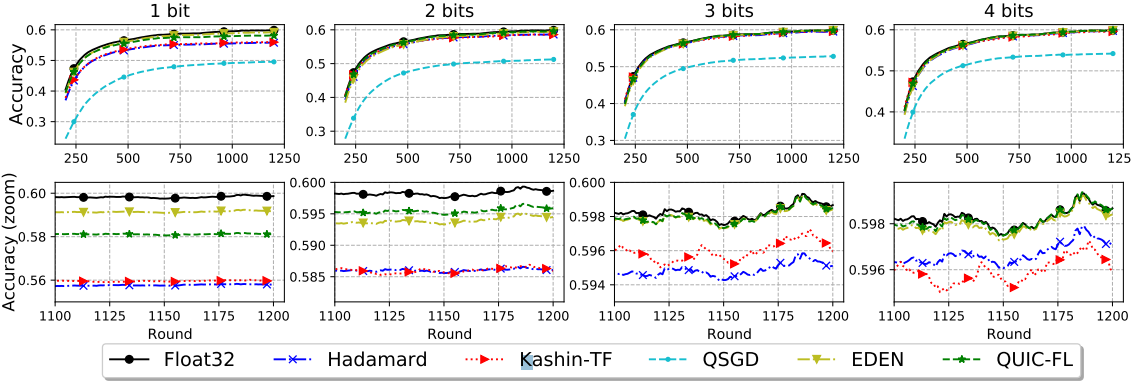
\includegraphics[width=\columnwidth]{images/nextword.png}
    \caption{\emph{FedAvg} over the Shakespeare next-word prediction task at
    various bit budgets (rows). Training accuracy per round reported as a
    rolling mean of 200 rounds. \cite{basat2023quicfl}}
    \label{fig:quic-fl-nextword}
\end{figure}

\begin{figure}[!ht]
    \centering
    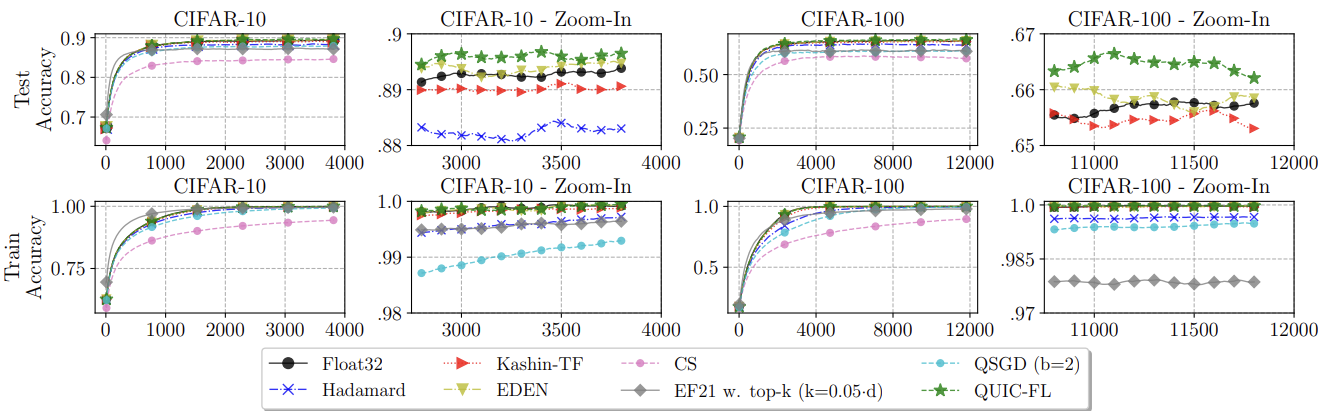
\includegraphics[width=\columnwidth]{images/results.png}
    \caption{Cross-device Federated Learning with Various Methods of Unbiased
    Quantization. \cite{basat2023quicfl}}
    \label{fig:quic-fl-acc}
\end{figure}

In the next-word prediction task in \autoref{fig:quic-fl-nextword}, QUIC-FL
performs the best for larger communication budgets, but not for smaller
communication budgets. QUIC-FL completes with EDEN for lower communication
budgets in terms of accuracy.

In the cross-device FL task, the CIFAR-10 and CIFAR-100 datasets are used.
QUIC-FL performs the best on both datasets in terms of test and train accuracy.
There is some tapering down with the number of rounds in test accuracy which
might be doubtful though.

\section{Future Works}
\label{sec:future}

After a thorough reading of the paper, the following concerns and suggestions
are raised by the authors of the paper as well as this report.
\begin{enumerate}
    \item (Open problem) Does using more than one RHT lead to better bounds?
    \item Can QUIC-FL be modified to perform better for cases using limited bits
    \(b\) and dimensions \(d\).
    \item Can the NMSE be lowered using a client-server feedback system?
    \item Security concerns of QUIC-FL.
    \begin{enumerate}
        \item Does the random transformation \(T\) in
        \autoref{alg:quic-fl-client} and \autoref{alg:quic-fl-server} act as a
        ``secret key''?
        \item What security guarantees does QUIC-FL have against various
        adversarial attacks?
    \end{enumerate}
    \item Can shared randomness be introduced to reduce the NMSE? What are the
    security and storage concerns regarding its use?
\end{enumerate}

\bibliography{references.bib}

\end{document}
